% % !TeX root = ../thuthesis-example.tex

\chapter{列表}

本章介绍另一种线性表:\textbf{列表}(list)。
列表和向量的区别在于,列表不要求在内存中占据的空间是连续的。
这一特点赋予了列表更大的灵活性,使列表的一些操作比向量效率更高;但同时,这一特点也让列表无法通过秩定位到内存地址,丧失了循秩访问的能力,从而在另一些操作上效率不如向量。\textit{本书会介绍列表是如何工作的,至于列表和向量的对比表格,希望读者在阅读后自己完成。}

\section{列表的结构}

列表不要求在内存中占据的空间是连续的,因此不能循秩访问,只能循位置访问:通过指向列表中某个元素的指针(也就是该元素的地址)来访问它。那么,如何获得一个元素的地址呢?首先,把所有元素的地址汇总在一张表看起来是可行的,但如果这么做的话,这张表本身如何存储就变成了一个新的问题。如果这个表使用向量存储,那么我们就放弃了列表的不连续的灵活性;如果这个表使用列表存储,那么就成为了一个嵌套的问题。所以,我们不能把所有元素的地址汇总在一张表,也就是说,我们不能采用\textit{集中式}的地址存储,需要采用\textit{分布式}的地址存储。

所谓分布式的地址存储,就是我们在每个元素处,同时存储它前一个和后一个元素的地址。这样,我们无论是从前往后还是从后往前,都能遍历整个列表。很明显,这样带来了一个坏处,就是我们只能“逐个”访问元素,而不能像向量那样根据任意的秩访问元素。这就是列表选择更大灵活性的代价。除此之外,列表还有一些其他的代价,比如每个元素处除了它本身的空间,还需要存两个地址,因而有可能需要付出比向量更大的空间(注意这里是有可能,因为向量的装填因子很低时,所造成的的空间浪费更大)。为了降低列表的空间浪费,有时我们会放弃存储前一个元素的地址,只存储后一个元素的地址。这种情况称为\textbf{单向列表}(forward list)或单链表,相对应地,同时存储前一个和后一个元素地址的情况称为\textbf{双向列表}(bidirectional list)或双链表。

\section{列表的节点}
\subsection{单向列表节点}
\label{lis:单向列表节点}
为了设计列表的抽象类,我们需要首先将列表中的每个元素抽象出来。列表中每个数据元素及其附加属性(即,前后元素的地址)组成了一个数据单元,或者称\textbf{节点}(node)。\textit{《计算机科学技术名词》}\cite{科学技术名词}\textit{认为“节点”是数据结构中数据元素的连接点或端点,而“结点”是计算机网络中的网络拓扑设备,并注明二者互为别称。本书不做区分。}本着从简到繁的精神,我们从单向列表的节点开始。

\begin{lstlisting}
template <typename T>
class ForwardListNode {
    T m_data;
    ForwardListNodeInst<T> m_next {};
public:
    ForwardListNode() = default;
    ForwardListNode(const T& data) : m_data(data) {}
    T& data() { return m_data; }
    ForwardListNodeInst<T>& next() { return m_next; }
};
\end{lstlisting}

以下对\lstinline{ForwardListNodeInst}这个类型进行说明。在邓书中,列表中的“位置”\lstinline{ListNodePos}直接被定义为\lstinline{ListNode}的裸指针类型。本书希望引导您学习更加丰富的现代C++编程范式,而智能指针是其中的重要一环,因此在本书的示例代码中,定义了三种\textit{代理}(proxy)类型~\cite{gregoire2021professional},分别对应裸指针、\lstinline{const}裸指针和\lstinline{std::unique_ptr}智能指针。其具体实现详见PointerProxy.ixx。
\begin{enumerate}
    \item 以\lstinline{Pos}结尾的类型是裸指针的代理。非空时,它表示一个实例的位置。
    \item 以\lstinline{ConstPos}结尾的类型是\lstinline{const}裸指针的代理。非空时,它表示一个实例的位置,且不允许通过此代理修改实例。
    \item 以\lstinline{Inst}结尾的类型是\lstinline{std::unique_ptr}智能指针的代理。非空时,它持有一个实例的所有权。
\end{enumerate}

上述三种类型与其代理的类型之间支持隐式转换,智能指针代理也可以被隐式转换为裸指针。这使得不了解智能指针的读者在使用本书的框架进行实验时,不需要经常通过\lstinline{get}方法转换为裸指针,也不需要经常用\lstinline{std::move}方法传递所有权。尽管如此,智能指针对您掌握现代C++的编程技巧是非常有益的,如果有时间,我仍然非常推荐您学习它。
本书的正文及示例代码都将以智能指针为主。

% 在示例代码中使用了一个代理类\lstinline{ForwardListNodeProxy},该类可以被隐式转换为裸指针,从而允许不熟悉智能指针的读者使用本书的示例代码完成实验。在本书的示例代码中,即使您删去了用于智能指针所有权传递的\lstinline{move}方法,改为像裸指针那样直接赋值,也不会影响代码的正确性。尽管如此,智能指针对您掌握现代C++的编程技巧是非常有益的,如果有时间,我仍然非常推荐您学习它。

回到单向列表的节点上。单向列表因为只有后向指针,所以我们将它声明为智能指针,让前一个节点具有后一个节点的所有权。这样,我们只要释放一个节点,就可以自动地释放掉它的所有后继。不过,这个想法看起来很美好,实际上却会出现问题。

\begin{figure}
  \centering
  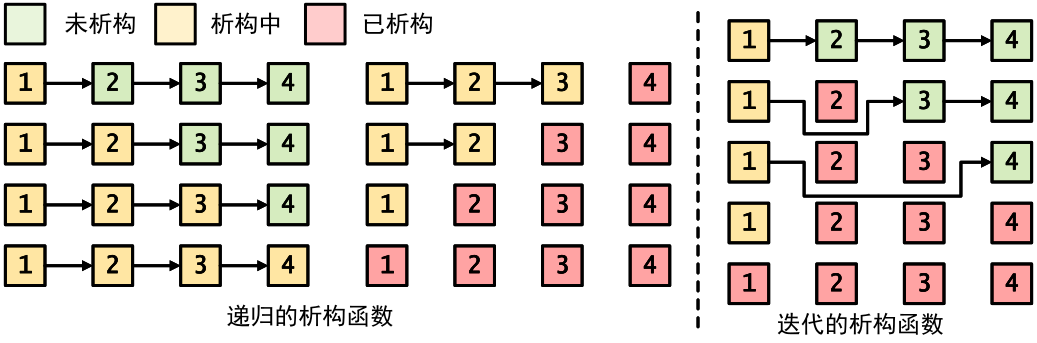
\includegraphics[width=\linewidth]{figures/lis8.pdf}
  \caption{列表节点的递归析构和迭代析构}
  \label{fig:lis8}
\end{figure}

对于规模为$n$的列表$L$来说,如果我们清空列表,释放它的第一个节点$L[0]$(请注意,虽然可以这样表记,但列表是不能循秩访问的),那么在$L[0]$的析构函数中会释放$L[0]$的后向指针,也就是$L[1]$。而在$L[1]$的析构函数中,又会释放$L[2]$,以此类推。如图\ref{fig:lis8}中的左图所示,黄色节点代表析构中的节点,可以看出在最后一个节点被析构的时候,前面所有的节点都在等待。对于规模为$n$的列表$L$,会触发$n$层析构函数的递归,当$n$非常大时,会引发栈溢出(stack overflow)错误。

因此,我们需要手动设计列表节点的析构函数,将析构函数的递归改为迭代,而不能依赖于\lstinline{std::unique_ptr}的自动释放空间。下面展示了一个迭代版本的析构函数,如图\ref{fig:lis8}的右图所示,它不会造成大量节点在析构中状态等待的情况。

\begin{lstlisting}
virtual ~ForwardListNode() {
    auto p { std::move(m_next) };
    while (p != nullptr) {
        p = std::move(p->m_next);
    }
}
\end{lstlisting}

\subsection{双向列表节点}

而当我们试图扩展单向列表到双向列表的时候,我们有两种选择。
\begin{enumerate}
    \item 让前向指针和后向指针共享节点的所有权,也就是两个指针都声明为\lstinline{std::shared_ptr}。这种做法过于浪费空间,因为\lstinline{std::shared_ptr}除了指针本身之外,还包括一个引用计数。
    \item 仍然保留只有后向指针拥有节点的所有权,也就是后向指针仍然是\lstinline{std::unique_ptr},而前向指针则使用不涉及所有权的裸指针。这种做法节约了空间,但会破坏前向指针和后向指针的对称性,提高算法设计难度。
\end{enumerate}

在本书中,采用后向指针单独拥有所有权,而前向指针使用裸指针的设计,因为对于基础数据结构而言,增加两个引用计数的成本是难以接受的。另一方面,本书通过将指针隐藏在代理类型下,一定程度解决了对称性的破坏问题。代理类之间的隐式转换可以让代码仍然具有良好的对称性。

\begin{lstlisting}
template <typename T>
class ListNode {
    T m_data;
    ListNodePos<T> m_prev {};
    ListNodeInst<T> m_next {};
public:
    ListNode() = default;
    ListNode(const T& data) : m_data(data) {}
    virtual ~ListNode() { /* ... */ }
    T& data() { return m_data; }
    ListNodePos<T>& prev() { return m_prev; }
    ListNodeInst<T>& next() { return m_next; }
};
\end{lstlisting}

如果您对智能指针不感兴趣,也可以使用裸指针改写本书中的这些节点类,变成您比较熟悉的形式。不要忘记\lstinline{delete}每一个创建的节点。

\subsection{哨兵节点}

在单向列表中,我们只能从前向后访问节点,所以,我们只需要知道指向第一个节点的指针,就可以从前向后依次访问所有节点。而在双向列表中,我们可以从两个方向访问节点,因此我们需要知道指向第一个节点和最后一个节点的指针,才可以从两个方向依次访问所有节点。

在邓书中,每个列表存在两个不存储实际数据的虚拟节点,称为\textbf{头哨兵节点}和\textbf{尾哨兵节点},或者简称为\textbf{头节点}(head)和\textbf{尾节点}(tail),用来标志列表的开始和结束。即使列表是空列表,这两个节点也存在。哨兵节点的引入使得许多实现得到了简化(simplify)和统一化(unify),比如前插(在一个节点之前插入新元素)不需要对第一节点进行特殊判定。\textit{在一些教材中介绍的列表是没有哨兵节点的,转而使用指向第一个节点和最后一个节点的裸指针来对头尾进行定位,称为头指针和尾指针。这不会影响到列表的功能,但有些功能的实现会略显复杂。在阅读完本章之后,您可以自己尝试写一个没有哨兵节点的列表,比较一下哪些功能的实现有所区别。}

\begin{lstlisting}
template <typename T>
class AbstractList : public AbstractLinearList<T, ListNodePos<T>> {
public:
    virtual ListNodePos<T> head() = 0;
    virtual ListNodePos<T> tail() = 0;
    virtual ListNodePos<T> insertAsNext(ListNodePos<T> p, const T& e) = 0;
    virtual ListNodePos<T> insertAsPrev(ListNodePos<T> p, const T& e) = 0;
    T& get(ListNodePos<T> p) override {
        return p->data();
    }
    void set(ListNodePos<T> p, const T& e) override {
        p->data() = e;
    }
};
\end{lstlisting}

根据头节点在第一个节点之前、尾节点在最后一个节点之后的特性,您可以自己补出此处没有展示的、继承线性表抽象类的\lstinline{first}和\lstinline{last}等方法。此外,我们将插入操作区分为了前插(插入为$p$的直接前驱)和后插(插入为$p$的直接后继)。因为后向指针和前向指针不是对称的,所以前插和后插也有一些区别。

单向列表的抽象类实现和双向列表基本一致。区别在于,单向列表不支持从后向前的访问;因此,单向列表不支持\lstinline{last}、\lstinline{back}和\lstinline{prev}等方法,我们需要将线性表抽象类中定义的这些方法设置为\lstinline{private}隐藏。

\begin{figure}
  \centering
  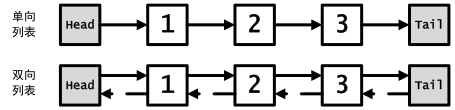
\includegraphics[width=0.8\linewidth]{figures/lis1.pdf}
  \caption{单向列表和双向列表}
  \label{fig:lis1}
\end{figure}

如图\ref{fig:lis1}所示,我们在单向列表和双向列表的两头各添加一个哨兵节点,代表所有权的智能指针用实线箭头表示,不涉及所有权的裸指针则用虚线箭头表示。由于哨兵节点的存在,用户总是可以知道列表的头和尾的位置。因此,即使在单向列表中,用户无法直接获得尾部(back)元素中的数据(需要从头节点向后依次遍历来寻找尾部),也无法直接删除尾部(pop back)的元素,但用户可以直接在尾部之后插入(push back)。如果没有尾节点的存在,则我们无法直接进行push back操作。在C++的标准库中,\lstinline{std::forward_list}就是这样设计的:它包含一个最简单、最节约空间的抽象,没有尾节点也不支持push back。

需要特别指出,\textit{哨兵节点仅仅用于列表的实现方法,而非列表的组成部分},因此在图\ref{fig:lis1}我们将它们用灰色表示。当我们具体讨论到某个列表$L[0]\to L[1]\to \dots\to L[n-1]$的时候,第一个节点$L[0]$和最后一个节点$L[n-1]$都是实际存储元素的节点,而非头节点或尾节点。在列表中,$L[0]$\textit{没有前驱};而在列表的具体实现中,我们\textit{可以认为}头节点是它的直接前驱以方便设计代码。

\section{插入、查找和删除}
\subsection{后插一个元素}
我们首先讨论后插。给定被插节点的位置$p$和待插入元素$e$,将元素$e$插入到列表中,使其对应的节点成为$p$的直接后继,这种类型的插入称为后插。对于双向列表,假设$p$原有的直接后继是$q$,则二者的指针连接形成$p\leftrightarrow q$的形式。我们希望将$e$插入到二者之间,形成$p\leftrightarrow e\leftrightarrow q$的形式。这里可以看出引入哨兵的好处。在引入哨兵节点之后,对于任何一个被插节点,它总是有直接后继$q$;当被插节点是最后一个节点时,$q$就是尾哨兵节点,而不需要进行特判。\textit{反过来,题目中如果遇到不含哨兵节点的情况(408中可能是默认的),则需要特别地考虑在首尾边界的情况,必要时进行特判。}

从宏观层面上来说,我们需要对$p$的后向指针、$q$的前向指针以及新生成的$e$的双向指针进行赋值,然而,这四个指针的赋值顺序需要仔细斟酌。这是设计列表算法的易错点,因为“拆散-重组”的过程不是一次性发生的,必定存在先后顺序。允许的顺序有许多种(所以不建议您背诵),但如果顺序错误,就有可能在拆散的过程中丢失了信息,导致无法进行重组。\textit{如果不熟练,那么当您设计这样的算法时,建议在纸上进行演算以确保“拆散-重组”过程是可行的。}

比如说,如果我们直接断开$p$到$q$的后向指针,将$e$接入,形成$p\rightarrow e\mid q$的形式,那么$q$会因为失去所有权而被智能指针自动回收(这种情况可以被生动地形容为“断链”)。因此,我们可以通过\lstinline{std::swap}交换智能指针的所有权,然后再将$q$连接到$e$的后向指针处。建立好$p\rightarrow e\rightarrow q$之后,再将前向指针补上。

\begin{lstlisting}
ListNodePos<T> insertAsNext(ListNodePos<T> p, const T& e) override {
    auto node { ListNodeInst<T>::make(e) };
    std::swap(p->next(), node);
    p->next()->next() = std::move(node);
    p->next()->prev() = p;
    p->next()->next()->prev() = p->next();
    ++m_size;
    return p->next();
}
\end{lstlisting}

\begin{figure}
  \centering
  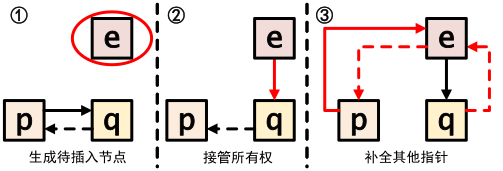
\includegraphics[width=0.8\linewidth]{figures/lis2.pdf}
  \caption{双向列表的后插}
  \label{fig:lis2}
\end{figure}

因为使用了交换语义,
上面的这种做法产生了比预期更多的赋值次数。
我们看到在上面的算法中,对于\lstinline{node}的重复赋值是\textit{不到位工作},它经历了$e$变化为$ q$、再变化为空的过程,而实际上可以让它一步到位地变化为空。于是,我们不应该从$p\rightarrow e\mid q$开始,可以从另一个后向指针,也就是$p\mid e\rightarrow q$开始。这样就能减少一次赋值。

从图\ref{fig:lis2}中可以看出,在后插的过程中,应当首先让$e$的后向指针接管$q$的所有权;而其他三项的赋值次序是可以随意的。当然,尽管次序可以随意,但在书写的时候仍然需要当心。比如,在$e$的后向指针接管$q$的所有权之后,我们不再能通过$p$的后向指针来找到$q$,只能通过$e$的后向指针来找到它。这些细小的注意点有时熟练的程序员也会忽略,因此在考试的时候借助图形和手工演算进行检查是有意义的。

\begin{lstlisting}
ListNodePos<T> insertAsNext(ListNodePos<T> p, const T& e) override {
    auto node { ListNodeInst<T>::make(e) };
    node->next() = std::move(p->next());
    node->next()->prev() = node;
    node->prev() = p;
    p->next() = std::move(node);
    ++m_size;
    return p->next();
}
\end{lstlisting}



单向列表的情况大同小异,只是减少了对前向指针赋值的操作。可以看出,在列表上做后插的时间复杂度和空间复杂度均为为$O(1)$。

\subsection{前插一个元素}
\label{sec:前插一个元素}
对于双向节点,前插的过程和后插大同小异。因为头哨兵节点的存在,我们总是可以找到$p$的直接前驱$q$,于是我们只需要在$q\leftrightarrow p$之间插入$e$,和前面的$p\leftrightarrow q$只有字母上的区别。\textit{您可以自己实现它,并检验自己的实现是否正确。请注意前向指针是裸指针,后向指针是智能指针。}当然,也可以直接用后插实现前插。

\begin{lstlisting}
ListNodePos<T> insertAsPrev(ListNodePos<T> p, const T& e) override {
    auto q { p->prev() };
    return insertAsNext(q, e);
}
\end{lstlisting}

对于单向列表,情况变得有些令人沮丧。因为单向列表中,我们无法使用前向指针,也就无法定位到$p$的直接前驱。那么,我们是否无法进行前插呢?是,也不是。我们可以用两种方法实现前插:
\begin{enumerate}
    \item 从头节点开始,沿着后向指针访问整个列表,寻找$p$的直接前驱,然后再采用和上面一样的方式进行前插。显而易见,如果$p$在列表中的秩是$r$,则该方法的时间复杂度高达线性的$\Theta(r)$。我们放弃循秩访问而使用列表,为的是允许操作不连续内存,从而在插入和删除的时候达到$O(1)$的常数复杂度;因此,这种方法虽然万无一失,但和我们的初衷背道而驰。
    \item 使用后插代替前插。我们首先找到$p$的直接后继$q$进行一次后插,形成$p\rightarrow e\rightarrow q$的形式,然后我们\textit{交换}$p$和$e$节点的值,形成$e\rightarrow p\rightarrow q$,如图\ref{fig:lis3}所示。这样在\textit{值}上实现了前插,但是在\textit{位置}上并没有实现前插。比如,如果原先外部有一个指针指向$p$,我们执行前插之后,这个指针并不知道$p$已经被$e$“偷梁换柱”了,它可能还以为自己指向的是$p$,从而产生不可估计的错误。因此,这种方法事实上损失了安全性。但是,毕竟它是一个$O(1)$的方法,我们也只能接受它,并期待用户正确地使用这个方法。
\end{enumerate}

\begin{figure}
  \centering
  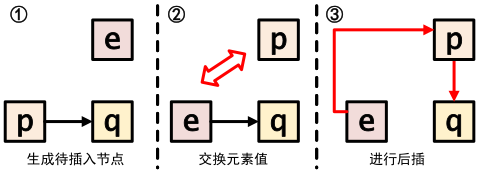
\includegraphics[width=0.8\linewidth]{figures/lis3.pdf}
  \caption{单向列表上使用后插代替前插}
  \label{fig:lis3}
\end{figure}

很显然,两种前插都存在一些问题,因此
C++标准库中的单向列表就不允许进行前插。
如果我们采用从头节点开始找前驱的方法进行前插,不了解它复杂度的用户可能会错误使用这个方法,造成用户写出的程序非常缓慢。这个问题曾经让旧标准的C++用户不胜其扰:在C++11之前,\lstinline{std::list}的获取规模方法\lstinline{size()}是$\Theta(n)$的,而用户很容易忘记这一点,从而造成用户应用程序时间效率的严重损失。如果我们使用后插代替前插,则会出现上述的指针指向混乱风险。在本书中为了让您了解单向列表实现前插的技巧,所以介绍了这两种方法,并在下面实现用后插代替前插的算法。在现实中设计程序时,应当避免这种高风险的设计。

回到使用后插代替前插的技术上。和上一节一样,我们注意到采用交换语义会引入不到位的赋值。在消除交换语义之后,一个可能的实现如下。

\begin{lstlisting}
ForwardListNodePos<T> insertAsPrev(ForwardListNodePos<T> p, const T& e) override {
    auto node { ForwardListNodeInst<T>::make(std::move(p->data())) };
    node->next() = std::move(p->next());
    p->next() = std::move(node);
    p->data() = e;
    if (m_tail == p) {
        m_tail = p->next();
    }
    ++m_size;
    return p;
}
\end{lstlisting}

前面讨论过,
如果原先外部有一个指针指向$p$,我们执行前插之后,这个指针并不知道$p$已经被替换了。我们无法保证用户使用的“外部指针”的安全性,但我们需要保证数据结构内部的指针的安全性。这个可能丧失安全性的指针就是尾节点指针\lstinline{m_tail}。当我们要在尾节点处进行前插(也就是push back)的时候,上述方法事实上进行了后插,并将原先的尾节点赋值为$e$。在这种情况下,我们需要将尾节点指针指向新的尾节点处。

另外,请注意这里必须对$p$中的数据使用移动语义,而不能使用复制语义,否则当$p$中的数据非常大(比如,一个被嵌套在列表里的向量)时,会引入大量的(非常数的)性能损失。

\subsection{查找一个元素}

无论是单向列表还是双向列表,查找元素的过程和无序向量都是一样的,只需要从前向后一个一个查找即可。因为不支持循秩访问的缘故,即使是有序列表,也不支持折半查找。\textit{您很容易自己实现顺序查找,下面是一个示例的实现。}

\begin{lstlisting}
ListNodePos<T> find(const T& e) const override {
    ListNodePos<T> p { m_head->next() };
    while (p != m_tail) {
        if (p->data() == e) {
            return p;
        }
        p = p->next();
    }
    return m_tail;
}
\end{lstlisting}

\subsection{删除一个元素}

列表删除是插入的逆操作。对于双向列表,假设被删除的节点为$p$,由于头节点和尾节点的存在,我们可以保证它存在直接前驱$q_1$和直接后继$q_2$。因此,我们需要将$q_1\leftrightarrow p \leftrightarrow q_2$变形为$q_1\leftrightarrow q_2$。显然,我们只需要对$q_1$的后向指针和$q_2$的前向指针各进行一次赋值。顺序仍然是重要的,但难度比插入降低了不少(因为2次赋值的顺序一共只有2种)。下面是一个可行的实现。

\begin{lstlisting}
T remove(ListNodePos<T> p) override {
    auto e { std::move(p->data()) };
    p->next()->prev() = p->prev();
    p->prev()->next() = std::move(p->next());
    --m_size;
    return e;
}
\end{lstlisting}

类似地,上面的做法也不适用于
单向列表的删除。对于单向列表,我们需要采用和前插相似的技术,首先找到$p$的直接后继$q_2$,以及$q_2$的后继$q_3$。我们在$p\rightarrow q_2\rightarrow q_3$上交换$p$和$q_2$节点上的值,从而在\textit{值}的角度,变成了$q_2\rightarrow p \rightarrow q_3$,然后重新复制$q_2$的后向指针,变为$q_2\rightarrow q_3$即可。双向列表和单向列表在删除节点上的区别如图\ref{fig:lis4}所示,请注意在双向列表的场合,当移交$q_2$的所有权之后,节点$p$会被智能指针自动释放(用灰色表示)。

图中$q_3$是虚线节点,这是因为
即使在存在尾节点的列表中,$q_3$仍然可能为空(\lstinline{nullptr})。如果$q_3$为空,那么$q_2$就是尾节点(在有哨兵的场合),交换元素之后我们会把原先的尾节点删除。所以,我们需要进行一次特判,在上述情况下让新的$q_2$成为新的尾节点。在消除了交换语义带来的不到位赋值之后,得到的一种示例程序如下所示。

\begin{lstlisting}
T remove(ForwardListNodePos<T> p) override {
    auto e { std::move(p->data()) };
    p->data() = std::move(p->next()->data());
    p->next() = std::move(p->next()->next());
    if (p->next() == nullptr) {
        m_tail = p;
    }
    --m_size;
    return e;
}
\end{lstlisting}

\begin{figure}
  \centering
  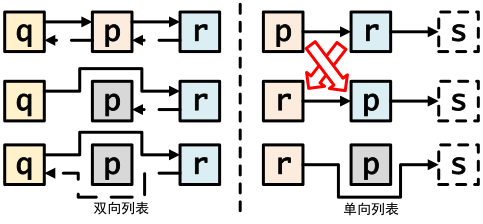
\includegraphics[width=0.8\linewidth]{figures/lis4.pdf}
  \caption{在列表中删除一个元素}
  \label{fig:lis4}
\end{figure}

和\ref{sec:前插一个元素}节一样,这里的尾节点指针\lstinline{m_tail}也是需要维护的“外部的指向节点的指针”。我们需要对这个指针重新赋值以避免安全性问题。在C++标准库的单向列表中,为了安全性考虑,只提供“删除后继”的方法\lstinline{erase_after}而不提供直接删除的方法。

从上面对插入、查找和删除的分析中可以看出,列表的三种基本操作完全不涉及规模。所以,如果不需要在$O(1)$时间里获取规模,那么列表是可以不记录这个属性的。不记录规模可以使列表在插入和删除时减少一次赋值,从而略微提高列表的性能。如果您自己实现了列表和单向列表,可以通过\textit{ListTest.cpp}和\textit{ForwardListTest.cpp}进行测试。

\subsection{实验:在头部和尾部连续插入元素}

随着三种基本操作分析完毕,我们可以开始对列表展开实验。这一节讨论在列表的头部和尾部连续插入元素的情况,代码可以在\textit{ListInsert.cpp}中找到。

在示例代码中,采用示例实现的向量、双向列表和单向列表类作为实验对象。您可以加入自己实现的版本,和它们的性能进行比较。
我们考虑两种环境。第一种是连续在头部插入元素,也就是每次插入的元素会成为线性表的第一个元素;另一种是连续在尾部插入元素,也就是每次插入的元素会成为线性表的最后一个元素。

这个实验表明,当在尾部连续插入元素时,向量的效率显著高于列表,但是单向列表并没有和双向列表之间有很大的差异。根据您的运行环境不同,向量和列表大致呈现一个数倍的性能差距,总体来说是常数的。需要特别指出的是,尽管在尾部\textit{连续}插入元素的测试中向量的性能高于列表,但对于\textit{单次}插入元素的过程则不一定。触发扩容时,向量单次插入元素的时间复杂度可达$\Theta(n)$,而列表是稳定的$O(1)$。这一点是列表的独特优势,在对响应时间稳定性有要求的场合下,向量的扩容变得不能接受,而列表的插入时间是可以保证很低的。

当在头部插入元素时,可以显著地看到,向量$\Theta(n^2)$的时间复杂度远高于列表$\Theta(n)$的时间复杂度,当$n=10^6$的时候向量的情况已经需要耗费几十秒(在笔者的计算机上);我们可以直接做一个判断,在这种情况下抛出一个\lstinline{error}拒绝执行,如下所示。

\begin{lstlisting}
void operator()(size_t n) override {
    if constexpr (is_base_of_v<AbstractVector<int>, Linear>) {
        if (n > 100000) {
            throw runtime_error { R"(Vector::push_front() is too slow for n > 100'000)" };
        }
    }
    for (size_t i { 0 }; i < n; ++i) {
        m_container.push_front(i);
    }
}
\end{lstlisting}

因为向量的耗时增长很快,我们在$n=10^5$量级已经可以看出它的性能,因此不需要花费大量的时间等待它在更大的规模上完成实验。这里采用了C++17引入的\lstinline{if constexpr}语法,从而实现在编译期判断。上面的代码对于以向量为参数的模板实例,会将\lstinline{if constexpr}内的判断编译进去;而对于以列表为参数的模板实例,则不会将\lstinline{if constexpr}内的判断编译进去;这个向量和列表的区分是编译期完成的,运行期不会再做判断。这一语法简洁清晰,可以用来替代C语言风格很容易被滥用的\lstinline{#ifdef}等条件编译命令。

\begin{table}
  \centering
  \caption{不同数据结构连续插入元素的耗时对比(单位:ms)}
  \begin{tabular}{cc|ccc}
    \toprule
    插入位置 & $n$ & 向量 & 列表 & 单向列表  
      \\
    \midrule
    尾部 & $10^4$ & 0 & 2 & 2 \\
    尾部 & $10^5$ & 1 & 22 & 21 \\
    尾部 & $10^6$ & 9 & 258 & 234 \\
    \midrule
    头部 & $10^4$ & 2 & 2 & 2 \\
    头部 & $10^5$ & 254 & 22 & 20 \\
    头部 & $10^6$ & 39167 & 222 & 198 \\
    \bottomrule
  \end{tabular}
  \label{tab:lis1}
\end{table}

在这个实验中,您还能发现的一点是,双向列表和单向列表在时间上的性能差异实际上非常小。双向列表虽然节点多了一个字段,但消耗的时间和单向列表相比,只有非常有限的增加,与此同时,它获得了从后向前访问的能力、更强的灵活性以及更好的安全性(关于安全性,在前插和删除的时候已经讨论过)。因此,除非性能要求苛刻或空间不足,否则都建议使用双向列表。

\subsection{实验:顺序删除和随机删除*}
\label{list:顺序删除和随机删除}
当我们连续地在列表中插入节点时,这些节点也会存在一定程度上的空间连续性,因为它们的空间是操作系统连续分配的。这会导致我们的实验并不能真实地反映出现实情况下的列表所包含的节点地址弱局部性这一特征。在这个实验中我们将会认识到,如果列表所包含的节点地址局部性很差,会对列表的性能造成很大的负面影响。

我们考虑下面的连续删除场景。代码可以在\textit{ListRemove.cpp}中找到。

\begin{lstlisting}
template <typename T>
class ContinuousPop : public Algorithm<void()> {
protected:
    List<T> L;
    Vector<ListNodePos<T>> V;
public:
    virtual void initialize(size_t n) = 0;
    void operator()() override {
        for (auto p : V) {
            L.remove(p);
        }
    }
};
\end{lstlisting}

在这个框架中,我们使用向量$V$来存储列表$L$的每一个节点的位置。通过初始化函数,我们让向量$V$成为顺序的或者随机的,然后,按照向量$V$中存储的节点次序依次删除列表中的元素。对于顺序存储的情况,每次向$L$加入元素后储存在$V$中即可,如下所示。对于随机存储的情况,可以在顺序存储之后增加一个\lstinline{std::shuffle}(我们在向量置乱的时候介绍过它)。

\begin{lstlisting}
// SequentialPop
void initialize(size_t n) override {
    L.clear();
    V.clear();
    for (size_t i { 0 }; i < n; ++i) {
        V.push_back(L.insertAsNext(L.last(), i));
    }
}
\end{lstlisting}

从这个例子中可以看到,当$n$比较小的时候,顺序删除和随机删除的性能基本一致;但当$n$比较大的时候,二者就会产生一个明显的差异。这个性能差异就是随机删除的局部性丧失引起的。

\begin{table}
  \centering
  \caption{顺序删除和随机删除的耗时对比(单位:ms)}
  \begin{tabular}{c|cc}
    \toprule
    $n$ & 顺序删除 & 随机删除
      \\
    \midrule
    $10^5$ &  21 & 25 \\
    $10^6$ &  190 & 285 \\
    $10^7$ &  2154 & 4649 \\
    \bottomrule
  \end{tabular}
  \label{tab:lis3}
\end{table}

在现实中,我们生成的列表可能不是以连续插入的形式分配内存的。因此,它可能天然就具有一个很差的局部性。这就意味着,现实中的列表在较坏的情况下有可能会更接近于本实验中随机访问的性能。结合上一个实验,我们意识到,列表和向量之间有着巨大的性能差距,甚至在数据结构规模较小的情况下,列表$O(1)$插入、删除的优势体现不出来,从时间消耗的角度上来说还不如$\Theta(n)$的向量操作。因此对于小型线性表,无论我们是否需要循秩访问、折半查找等向量特性,都应该优先使用向量而不是列表。

\subsection{实验:倒置列表}

当在向量上设计算法的时候,由于向量循秩访问的特性,我们可以对秩进行运算,从而快速、精准地找到某个元素。一个典型的例子就是折半查找。循秩访问使得向量中的元素地位比较“平等”;而在列表的场合,循位置访问使得列表中的元素地位比较“不平等”,比较“任人唯亲”。比如,从头节点出发访问列表中的一个元素时,所需要消耗的时间会和被访问元素的位置相关;越接近头部的元素,访问需要的时间越短。

我们可以站在更高的层次,理解
列表只能直接访问首尾两端、以及循位置访问“任人唯亲”的特性:列表是\textbf{线性递归定义}的。具体来说,列表可以被这样定义:
\begin{enumerate}
    \item $\emptyset$是列表(空列表,没有元素)。
    \item 设$x$是一个节点,$L$是一个列表,则$x\to L$是列表($x$的后向指针指向$L$的第一个节点)。
\end{enumerate}

这个定义具有和《绪论》章所述递降法相似的形式,它也就意味着列表适合使用减治思想设计算法。首先,我们研究递归边界(空列表)的情况;其次,对于规模为$n$的列表,我们将第一个节点提取出来,递归地研究后$n-1$个节点组成的子列表,再和第一个节点进行合并。对称地,我们可以想到列表具有另一个定义:
\begin{enumerate}
    \item $\emptyset$是列表(空列表,没有元素)。
    \item 设$x$是一个节点,$L$是一个列表,则$L\to x$是列表($L$的最后一个节点的后向指针指向$x$)。
\end{enumerate}

这一定义同样可以引出一种减治算法的设计。它和前一种定义的区别在于,平凡项$x$在减治项$L$的头部还是尾部。对于双向列表来说,头部减治和尾部减治是等价的,提取出平凡项$x$都只需要$O(1)$的时间。当然,我们需要注意,减治递归算法应用在列表上时,递归深度高达$\Theta(n)$,这不但导致了较高的空间复杂度,同时在$n$较大时很可能引发栈溢出错误;因此在设计完成减治算法之后,应当尽可能将其修改为迭代算法。

单向列表的头部和尾部不具有对称性,因此情况会有所不同。考虑单向列表$L[0]\to L[1]\to L[2]\to \dots \to L[n-1]$。当在头部进行减治时,只需要$O(1)$的时间就可以找到$L[0]$;而在尾部进行减治时,需要$\Theta(n)$的时间才能找到$L[n-1]$。看起来单向列表应当总是在头部进行减治,然而事实却不一定是如此。本节将以倒置列表为例子,对两种减治方法进行比较。代码可以在\textit{ListReverse.cpp}中找到。为了便于和双向列表上的算法进行对比,我们总是传入双向列表\lstinline{List<T>&}作为参数类型,并在设计单向列表算法的时候不使用涉及前向指针的方法。

对于双向列表的倒置,我们可以直接从头尾两个方向遍历,交换对称的两个节点的数据域。这种做法和向量上的做法一致,也可以使用\lstinline{std::reverse}。
\begin{lstlisting}
// ReverseBasic
void operator()(List<T>& L) override {
    auto head { L.head() };
    auto tail { L.tail() };
    for (auto size { L.size() }; size >= 2; size -= 2) {
        head = head->next();
        tail = tail->prev();
        std::swap(head->data(), tail->data());
    }
}
\end{lstlisting}

下面讨论单向列表,
首先考虑在头部进行减治的情况。按照减治的思想,在将$L[0]$摘出列表之后,把从$L[1]$开始的剩余列表反转,然后再进行合并:把被摘出的$L[0]$接到反转后的剩余列表的尾部,如图\ref{fig:lis9}中的左图所示。



\begin{lstlisting}
// ReverseReduceAtHead
void operator()(List<T>& L) override {
    if (L.size() < 2) {
        return;
    }
    auto first { L.pop_front() };
    (*this)(L);
    L.push_back(first);
}
\end{lstlisting}

\begin{figure}
  \centering
  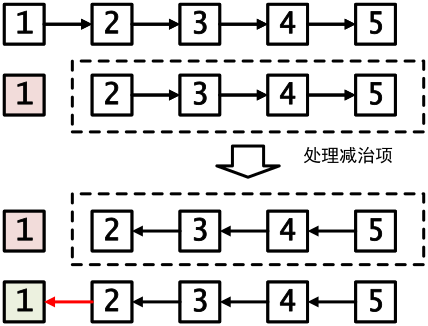
\includegraphics[width=0.9\linewidth]{figures/lis9.pdf}
  \caption{利用头部减治和尾部减治倒置列表}
  \label{fig:lis9}
\end{figure}

它的时间复杂度和空间复杂度均为$\Theta(n)$。
这个算法并不是尾递归,这意味着我们将它改写成迭代的时候会遇到困难。这一困难来自于我们在做递归调用的时候,需要保存当前递归实例摘出的元素\lstinline{first}。当我们进行到最后一层递归调用的时候,需要保存之前每一次摘出的元素,这就意味着不可避免地需要$\Theta(n)$的空间。这也就意味着,将此方法改写为迭代之后,几乎和下面的“极端”做法等价。

\begin{lstlisting}
// ReverseMove
void operator()(List<T>& L) override {
    Vector V(L.size());
    move(begin(L), end(L), begin(V));
    reverse(begin(V), end(V));
    move(begin(V), end(V), begin(L));
}
\end{lstlisting}

这个做法的时间复杂度和空间复杂度同样都是$\Theta(n)$。它将所有元素移动到一个辅助向量里,在向量里面倒置,再移动回列表里。

无论是命题者还是我们自己,都很难接受这样的算法。从刚才的分析中已经可以发现,影响空间效率的主要原因是,单向列表只有后向指针。当在头部进行减治的时候,被提取出来的$L[0]$彻底和$L[1$:$n]$断开,无法通过$L[1$:$n]$上的指针找到$L[0]$,从而必须要额外的空间来存储它。于是就可以想到,是否可以利用单向列表的\textit{不对称性},采用在尾部进行减治的策略设计算法?答案是肯定的。当在尾部进行减治的时候,我们可以先处理$L[0$:$n-1]$,然后利用$L[n-1]$的后向指针直接找到$L[n]$。下面展示了一个示例代码。

\begin{lstlisting}
template <typename T>
class ReverseReduceAtTail : public ReverseForwardList<T> {
    ListNodeInst<T> reverse(ListNodeInst<T>& start, size_t size) {
        if (size == 1) {
            return move(start->next());
        }
        auto last { reverse(start, size - 1) };
        auto tmp { move(last->next()) };
        last->next() = move(start);
        start = move(last);
        return tmp;
    }
public:
    void operator()(List<T>& L) override {
        auto old_first { L.first() };
        auto start { move(L.head()->next()) };
        auto last { reverse(start, L.size()) };
        L.head()->next() = move(start);
        old_first->next() = move(last);
    }
};
\end{lstlisting}

如图\ref{fig:lis9}中右图所示,上述算法中将减治项和平凡项合并的过程,就是在\lstinline{start}、\lstinline{last}和红色指针之间进行了一个轮换。
这份代码很容易被改写为迭代,因为它在进行递归调用处理减治项的时候,并不需要存储合并的时候需要用到的变量。我们可以使用固定的变量\lstinline{start}和\lstinline{size},作为每次递归调用的参数,并使用固定的变量\lstinline{last}存储每次递归调用的返回值。一个示例的迭代写法如下所示。

\begin{lstlisting}
// ReverseReduceAtTailIterative
void operator()(List<T>& L) override {
    auto old_first { L.first() };
    auto start { move(L.head()->next()) };
    auto last { move(start->next()) };
    for (auto size { L.size() }; size > 1; --size) {
        auto tmp { move(last->next()) };
        last->next() = move(start);
        start = move(last);
        last = move(tmp);
    }
    L.head()->next() = move(start);
    old_first->next() = move(last);
}
\end{lstlisting}

上述算法的时间复杂度为$\Theta(n)$,空间复杂度为$O(1)$。此外,这是一个针对指针域进行操作的算法,在整个算法过程中,只有各个后向指针的指向发生了变化,而每个节点内部的数据域没有变化,也没有创建或删除节点。上面介绍在头部进行减治的算法时涉及到了创建和删除节点,您可以自己尝试对示例代码进行修改,让它也成为一个针对指针域进行操作的算法。

\begin{table}
  \centering
  \caption{倒置列表算法的耗时对比(单位:ms)}
  \begin{tabular}{c|ccccc}
    \toprule
    $n$ & \thead{数据域\\Basic} & \thead{数据域\\转移到向量} & \thead{指针域\\头部减治\\递归} & \thead{指针域\\尾部减治\\递归} & \thead{指针域\\尾部减治\\迭代}  
      \\
    \midrule
    $10^3$ &  0 & 0 & 0 & 0 & 0 \\
    $10^4$ &  0 & 0 & 栈溢出 & 栈溢出 & 1 \\
    $10^5$ &  2 & 12 & 栈溢出 & 栈溢出 & 16 \\
    $10^6$ &  25 & 134 & 栈溢出 & 栈溢出 & 190 \\
    $10^7$ &  248 & 1142 & 栈溢出 & 栈溢出 & 1617 \\
    \bottomrule
  \end{tabular}
  \label{tab:lis2}
\end{table}


另一方面,之前介绍的ReverseBasic算法,逐个交换双向列表中对称的节点上的数据,是针对数据域进行操作的算法。在整个算法过程中,只有各个节点内部的数据域发生了变化,而没有改变每个节点的指针指向关系,也没有创建或删除节点。

\textbf{针对指针域}和\textbf{针对数据域},是设计列表算法时的两种不同路径。针对指针域的算法将列表上的节点当做一个整体,通过修改指针来改变节点在列表中的顺序。针对数据域的算法则将列表当做一个访问受限(只能访问已知位置的直接前驱和直接后继)的向量处理。如果一个向量上的算法没有涉及循秩访问,那就可以原封不动地迁移到列表上。涉及循秩访问的算法如折半查找则不适用。这种做法显得非常投机取巧,但效率却不一定低,在现实程序开发中不失为一种选择。为了避免考生投机取巧,试卷经常会强制要求只能针对指针域设计算法。请您根据自己对双向列表的理解,将上面的尾部减治算法改为双向列表的版本。

在实际解题时给出的列表,有可能无法直接通过\lstinline{size}方法获取规模,此时有两种方法可以解决。其一是直接遍历一遍整个列表做个统计,因为不会影响时间复杂度和空间复杂度,这种做法通常是可行的。其二是改变迭代的终止条件(递归边界)为不涉及规模的形式,在不同的算法中这一修改会有所不同。您可以尝试对ReverseBasic以及尾部减治算法进行修改,使其不涉及列表的规模。

\section{列表的归并排序}

\subsection{基于值的归并排序}

本节讨论在列表上做归并排序,这是一个比较复杂的列表操作。
一种基本的思路是基于\textit{值}的归并排序,即之前在\ref{sec:归并排序}和\ref{sec:自下而上的归并排序}节使用的归并排序。因为从迭代器的观点看,向量和列表作为线性表具有高度的相似性,所以无论是双向列表还是单向列表,都可以使用相同的代码进行归并排序。唯一的区别在于向量的迭代器支持随机访问,而列表无法支持这一点。因此,在我们想要找到中点的时候,向量的版本可以直接使用左边界和右边界的平均值,而列表的版本只能传入一个规模并手动向前依次迭代;幸运的是,迭代的时间是$\Theta(n)$的,和归并的时间相同,因此不会引入更高的时间复杂度。

\subsection{基于指针的归并排序*}

显然,上面这种归并排序没能发挥列表的特点。在归并的时候,没有必要使用快慢指针,而是可以充分利用列表的灵活性,达到不需要辅助空间的效果。比如,原先的列表$L$可以分成$L_1$和$L_2$两部分,现在为了对列表$L_1\rightarrow L_2$,我们可以首先将它切断成两个独立的列表$L_1$和$L_2$。随后,令$L=\emptyset$清空,依次比较$L_1$和$L_2$的首节点,将较小的节点\textit{移动}到$L$的末尾。全部移动结束后,就完成了对$L$的归并。\textit{这是一个相当有挑战性的工作,几乎达到了笔试中手写代码的最大可能难度,需要对列表有深刻的理解才能写出来。非常建议您进行这项尝试。这里的示例程序仍然有进一步优化的空间。}

上一小节讨论的基于值的归并排序,在整个排序过程中没有修改任何节点的相对位置,只是改动了每个节点里的数据元素的值。因此这个版本的实现和向量相同,因为向量也不能改变数据单元的相对位置,向量中相对位置和绝对位置(地址)是统一的。而这里的归并排序,则在整个排序过程中,每个节点的值都没有被修改,被改动的只有节点的前向和后向指针,从而改变节点的相对位置。这是在邓书中介绍的版本,它的原理仍然是归并排序,但归并的实现和向量的版本完全不同。
\begin{figure}[H]
  \centering
  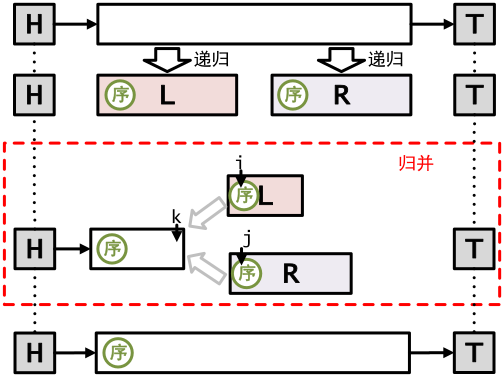
\includegraphics[width=0.95\linewidth]{figures/lis5.pdf}
  \caption{基于指针的归并排序}
  \label{fig:lis5}
\end{figure}

哨兵节点在这个版本的归并排序里会产生麻烦,因为它们会破坏拆分后的列表结构。如图\ref{fig:lis5}所示,如果在拆分列表前不分离哨兵节点,则拆分后的前后两段,一个只有头节点,一个只有尾节点,需要各自单独判断;如果先分离哨兵节点再拆分,则两段都既没有头节点也没有尾节点,不需要单独判断。当数据区域被排序完成之后,再将头尾节点接入即可。在归并的时候,示例代码里使用了一个哑节点(dummy)来起到临时头节点的功能,这对于不带头节点的列表算法设计是常用的技术。在归并的过程中,哑节点不是列表整体的头节点,而是正在被归并的这一段的临时头节点,归并结束之后,排好序的这一段会和哑节点分离。您也可以直接使用被分离下来的头节点担任这一职能(示例代码中为了展示哑节点的作用没有这么做)。

% 为了实现这个版本的归并排序,我们首先考虑将一个列表切断为两个独立的列表。考虑列表$h\rightarrow L_1\rightarrow L_2\rightarrow t$,其中$h$和$t$分别是头节点和尾节点。那么,我们需要从$h$出发经过$\frac{n}2+1$长度,找到$L_2$的第一个节点$L_2[0]$。那么,我们可以将$L_1$认为是头节点为$h$、尾节点为$L_2[0]$的一个列表,从而可以对它进行递归的归并排序。同理,我们可以从$h$出发经过$\frac{n}2$长度,找到$L_1$的最后一个节点$L_1[-1]$,认为$L_2$是头节点为$L_1[-1]$、尾节点为$t$的一个列表进行递归的归并排序。进行递归之后,我们再将$h,L_1,L_2,t$切分开来进行归并,如图\ref{fig:lis5}所示。

\begin{lstlisting}
template <typename T, template<typename> typename List>
    requires std::is_base_of_v<AbstractList<T>, List<T>>
class ListMergeSort : public AbstractSort<T, List> {
    using Pos = ListNodePos<T>;
    using Inst = ListNodeInst<T>;
    Inst dummy { Inst::make() };
    Inst& forward(Pos from, size_t step) {
        for (size_t i { 1 }; i < step; ++i) {
            from = from->next();
        }
        return from->next();
    }
    void connect(Pos& prev, Inst& next) {
        next->prev() = prev;
        prev->next() = std::move(next);
        prev = prev->next();
        next = std::move(prev->next());
    }
    void merge(Inst& L1, Inst& L2) {
        Pos L { dummy };
        while (L1 && L2) {
            if (this->cmp(L1->data(), L2->data())) {
                connect(L, L1);
            } else {
                connect(L, L2);
            }
        }
        if (L1) {
            L->next() = std::move(L1);
        } else {
            L->next() = std::move(L2);
        }
        L1 = std::move(dummy->next());
    }
    void mergeSort(Inst& head, size_t size) {
        if (size < 2) return;
        auto mi { std::move(forward(head, size / 2)) };
        mergeSort(head, size / 2);
        mergeSort(mi, size - size / 2);
        merge(head, mi);
    }
protected:
    void sort(List<T>& L) override {
        if (L.empty()) {
            return;
        }
        auto first { std::move(L.head()->next()) };
        auto tail { std::move(L.tail()->prev()->next()) };
        mergeSort(first, L.size());
        forward(first, L.size() - 1)->next() = std::move(tail);
        L.head()->next() = std::move(first);
    }
};
\end{lstlisting}

上面的这个做法因为只需要调用\lstinline{forward}来从前向后地移动指针,所以也同样支持单向列表。将所有对前向指针的赋值删去即可。

\subsection{实验:归并排序的性能差异*}

基于指针的归并排序,将空间复杂度从$\Theta(n)$降低到了$\Theta(\log n)$(一定要注意递归本身的空间复杂度,不能误以为是$O(1)$),那么显然地,它会在时间上有所损失。为了评估归并排序的性能差异,我们设计了一个实验。代码可以在\textit{ListMergeSort.cpp}中找到。

\begin{table}
  \centering
  \caption{归并排序的耗时对比(单位:ms)}
  \begin{tabular}{c|cccccccc}
    \toprule
  $n$ & \thead{向量\\自上而下} & \thead{向量\\自下而上} & \thead{顺序\\列表\\自上而下\\基于值} & \thead{顺序\\列表\\自下而上\\基于值} & \thead{顺序\\列表\\自上而下\\基于指针} & \thead{随机化\\列表\\自上而下\\基于值} & \thead{随机化\\列表\\自下而上\\基于值} & \thead{随机化\\列表\\自上而下\\基于指针}  
      \\
    \midrule
  $10^4$ &  11 & 12 & 14 & 15 & 16 & 16 & 20 & 16 \\
  $10^5$ &  143 & 148 & 203 & 254 & 242 & 287 & 448 & 289 \\
  $10^6$ &  1749 & 1759 & 2415 & 2917 & 3252 & 4105 & 5299 & 3585 \\
    \bottomrule
  \end{tabular}
  \label{tab:lis4}
\end{table}


我们对比三个归并排序,分别为用基于值的方法实现的归并排序(自上而下和自下而上版本),以及基于指针的归并排序。实验结果表明,和向量的情况不同,在列表的场合,自下而上的归并排序消耗的时间会显著高于自上而下的归并排序。这是因为,自上而下版本的一些归并段的左右端点来自递归调用的参数,只有中点需要自己找;自下而上版本因为没有递归,所以在已知左端点的情况下,需要自己找中点和右端点。在循秩访问的向量中,这只是多了一次加法,时间消耗可以忽略不计;而在循位置访问的列表中,找端点需要循着后向指针一个一个找,时间消耗就明显增加了。自上而下的版本用时明显比向量归并排序多,一定程度上也来自于这个原因。

另一个影响归并排序效率的重要因素来自于局部性。实验中提供了一个\lstinline{shuffle}方法,用于将列表中的节点随机打乱。您可以观察调用了该方法和不调用的区别。在不调用\lstinline{shuffle}的情况下,自下而上的版本就会和自上而下版本有一定的差距,而基于指针的版本在$n$较大的情况下会更慢。这是因为不随机打乱的时候,列表中的节点是连续生成的,因此基于值的排序能利用到局部性,而基于指针的排序在排序过程中会将节点次序打乱从而丧失局部性。

但在调用了\lstinline{shuffle}的情况下,情况会发生变化。所有版本的列表归并排序都会因为损失局部性而性能降低。由于循着后向指针一个一个找的过程没有了局部性,自下而上版本和自上而下版本的差距会进一步拉大。基于指针的版本因为移动指针本来就会破坏局部性,受到的影响比较小。

\section{循环列表}

\textbf{循环列表}(circular list)基于循环链表,后者是普通的、线性的链表的一个变体。简单地说,循环列表就是舍弃了头节点和尾节点,让第一个节点$L[0]$的前向指针指向最后一个节点$L[-1]$,让最后一个节点$L[-1]$的后向指针指向第一个节点$L[0]$,首尾相连,形成的环状结构。循环列表同样可以分为单向循环列表和双向循环列表。循环列表的三种基本操作和本章中介绍的普通线性列表几乎完全一致,所以不再赘述。邓书中也删除了这部分内容。

\begin{figure}
  \centering
  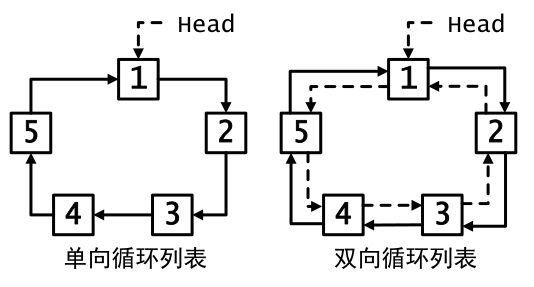
\includegraphics[width=0.8\linewidth]{figures/lis6.pdf}
  \caption{循环列表}
  \label{fig:lis6}
\end{figure}

图\ref{fig:lis6}展示了单向循环列表和双向循环列表的结构。由于需要保证列表的节点首尾相连,所以无法在循环列表的环上嵌入哨兵节点。图中的\lstinline{head}称为\textbf{头指针},它是一个指向列表中第一个元素的裸指针;类似地,也可以(可选地)用一个\textbf{尾指针}指向列表中的最后一个元素。

注意到,如果循环列表中只有一个元素,那么它的后向指针(双向循环列表中,也包括前向指针)将指向自己,因此它持有自身的所有权。您可以通过画图演算发现,使用本章中介绍的普通线性列表的删除方法,删除循环列表中唯一的一个元素时,会无法释放这个唯一元素的空间。因此,对最后一个元素进行删除的时候需要进行特判。如果您实现了循环列表,可以通过\textit{CircularListTest.cpp}进行测试。

循环列表的主要特征是:循环列表上的指针沿着前向指针或后向指针走下去,就可以在列表上\textit{无限轮询}每个节点。这种无限轮询的特点使它在《网络原理》和《操作系统》这两门学科“持续性维护”的情景中有用武之地,但在《数据结构》中不常用。在\textit{CircularListIterate.cpp}中您可以看到无限轮询的例子。

\section{静态列表}

\subsection{静态列表的结构}

\textbf{静态列表}(static list)指的是基于数组实现的列表(或者也可以基于向量实现,从而允许扩容)。列表在建立的时候,申请一块连续的内存,所有的节点都存在这部分内存中。与向量有所区别的是,节点的相对位置可以和它们在数组里的位置不同。在静态列表中,前向指针和后向指针往往用所基于的数组(向量)中的下标代替,因此,静态列表虽然本质上是一种循位置访问的结构(列表),但它的位置是用秩表示的,因为列表中的节点存在数组或向量里。

和动态分配内存的动态列表相比,由于装填因子的问题,静态列表需要消耗更多的空间,所以它非常不常用(仅出现在不提供指针/引用语法的古代编程语言中),邓书删除了这部分内容,也几乎不会出现在考试中。但在机试里,由于动态分配内存可能会引起时间消耗上的不确定性,并且机试题目给定的空间几乎总是绰绰有余的,所以静态列表仍然有发挥的空间。

单链/双链、线性/循环、动态/静态,这三对关系是相互独立的,可以组成8种不同结构的列表实现。在本节将以双链、线性为例,介绍静态列表的实现方法。为了支持扩容,这里基于向量实现。由于静态列表和动态列表非常相似,这里只介绍静态列表的特有特点。

\subsection{静态列表上的节点}

和动态列表不同,静态列表用来存储前向指针和后向指针的类型变成了秩。
\begin{lstlisting}
template <typename T>
class StaticListNode {
    T m_data;
    Rank m_prev { 0 };
    Rank m_next { 0 };
};
\end{lstlisting}

对于秩而言,我们需要指定特殊值用来对应指针情形中的空指针。在这里,我们认为秩为0表示指向空;因此在实现静态列表的时候,我们不能使用秩为0的数据单元来存放数据,否则会产生混淆。当然,也可以规定一个不可能出现的值(比如-1)。除了秩为0的单元外,我们还需要规定固定的单元用来存放头节点和尾节点。

\begin{lstlisting}
template <typename T>
class StaticList : public AbstractStaticList<T> {
    Vector<StaticListNode<T>> m_data {};
    const static Rank m_head { 1 };
    const static Rank m_tail { 2 };
    StaticListNode<T>& getNode(Rank r) override {
        return m_data[r];
    }
};
\end{lstlisting}

这里,我们采用了一个\lstinline{getNode}方法在秩和位置之间建立联系。静态列表的操作和动态列表相比大同小异,因为不需要考虑智能指针的所有权问题,静态列表可以更加随意一些,比如,下面是静态列表的后插实现。

\begin{lstlisting}
Rank insertAsNext(Rank p, const T& e) override {
    Rank r { m_data.size() };
    m_data.push_back(StaticListNode<T>(e, p, getNode(p).next()));
    getNode(p).next() = r;
    getNode(getNode(r).next()).prev() = r;
    return r;
}
\end{lstlisting}

\subsection{在静态列表上删除一个元素*}
\label{lis:在静态列表上删除元素}
如果我们按照动态列表的方法在静态列表上删除,可以得到下面的算法。

\begin{lstlisting}
T remove(Rank r) override {
    T e { std::move(getNode(r).data()) };
    getNode(getNode(r).prev()).next() = getNode(r).next();
    getNode(getNode(r).next()).prev() = getNode(r).prev();
    return e;
}
\end{lstlisting}




上述算法存在一个致命的问题:被删除的节点的内存无法被释放。
因为被删除的节点在向量$V$中,所以不能直接释放内存。
所以,需要将被删除的节点从向量$V$中删除,以释放$V$中的空间,使其可以被分配给其他节点。
然而,直接调用向量的删除元素方法也是不行的。因为删除$V[0$:$n]$中的一个节点$V[r]$,会导致它的后缀$V[r+1$:$n]$整体前移。$V[r+1$:$n]$的前移会导致这些节点的秩发生变化,如果其他节点的前向或后向指针指向了它们,则需要更新这些指针。所以,如果用从$V$中删除节点的方式来清理内存,则删除一个节点的时间复杂度高达$\Theta(n-r)=O(n)$,这是列表所不能允许的。


为了将删除节点的影响降到最低,则希望$r$越大越好。当$r=n-1$(被删除的节点在向量末尾)时,$\Theta(n-r)=O(1)$,这是列表所理想的结果。
因为列表的元素次序和$V$中的元素次序无关,所以您可以很自然地想到,只需要将$V[r]$交换到$V[n-1]$,就可以顺利在$O(1)$的时间内删除了。一个可能的实现原理如图\ref{fig:lis7}所示。

\begin{figure}[H]
  \centering
  \includegraphics[width=0.8\linewidth]{figures/lis7.pdf}
  \caption{在静态列表上删除一个元素}
  \label{fig:lis7}
\end{figure}

\begin{lstlisting}
T remove(Rank r) override {
    T e { std::move(getNode(r).data()) };
    getNode(getNode(r).prev()).next() = getNode(r).next();
    getNode(getNode(r).next()).prev() = getNode(r).prev();
    Rank s { m_data.size() - 1 };
    if (r != s) {
        getNode(r) = std::move(getNode(s));
        getNode(getNode(r).prev()).next() = r;
        getNode(getNode(r).next()).prev() = r;
    }
    m_data.pop_back();
    return e;
}
\end{lstlisting}




对于元素次序不重要的向量结构,在执行删除时,可以将被删除的元素移动到向量末尾再删除,可以将删除操作的时间复杂度从$\Theta(n-r)$降低为$O(1)$,这是一个常用的技巧。在后面的章节中还会再次出现。当然,根据我们在\ref{sec:前插一个元素}节中的经验,这种对值的直接操作是不安全的。所以,如果确保空间足够,也可以选择静态列表在删除元素的时候不释放空间:在机试的时候通常都是这么做的。

如果您实现了静态列表,可以使用\textit{StaticListTest.cpp}进行测试。

\section{本章小结}
和向量相比,列表的链式结构显得不那么直观,在列表上进行插入、删除等操作时对指针的多次赋值,对初学者而言颇有难度。以列表为背景的算法设计题也常常从链式结构本身的性质入手,重点考察学生对于通过指针赋值进行链表操作的能力。在具体的题目中,有无头节点、有无尾节点、单向还是双向、顺序还是循环等因素,都会影响链表算法的具体实现,因此记忆代码是不可行的,应当理解设计列表操作的一般方法。

本书采用智能指针实现列表,为读者提供了一个不同于教材的视角:所有权视角。每个节点被且仅被一个智能指针持有所有权,我希望这一特性使得读者能够在设计链表操作的时候能够有迹可循(尽管遇到的题目使用的是裸指针)。下面列出了本章的一些学习目标。

\begin{enumerate}
    \item 您学会了绘制列表的指针关系图,通过图形设计算法。
    \item 您学会了采用后向智能指针控制列表节点所有权,并能从所有权的视角触发设计指针赋值操作序列,注意避免“断链”和更新“外部指针”。
    \item 您了解到列表作为线性递归定义的数据结构,适合使用减治策略设计算法。
    \item 您了解到设计列表上的算法时,可以有针对数据域和针对指针域两种路径。
    \item 您了解到对没有头节点的列表设计算法时,可以使用哑节点作为临时头节点。
\end{enumerate}

\begin{table}
  \centering
  \caption{向量、列表和单向列表的对比}
  \begin{tabular}{c|ccc}
    \toprule
  & 向量 & 双向列表 & 单向列表
      \\
    \midrule
存储连续 & √ & × & × \\
性能稳定 & × & √ & √ \\
增删灵活 & × & √ & 〇 \\
位置安全 & 〇 & √ & × \\
节约空间 & √ & × & 〇 \\
    \bottomrule
  \end{tabular}
  \label{tab:lis5}
\end{table}

向量和列表的区别也是一个重要的问题。本书从插入、删除和归并排序等几种典型场景出发,对向量、双向列表和单向列表的区别作出了分析。在表中提供了几个视角,您应当根据自己的理解,列出更加全面的对比表格。

% \chapter{数学符号和公式}

% \section{数学符号}

% 中文论文的数学符号默认遵循 GB/T 3102.11—1993《物理科学和技术中使用的数学符号》
% \footnote{原 GB 3102.11—1993,自 2017 年 3 月 23 日起,该标准转为推荐性标准。}。
% 该标准参照采纳 ISO 31-11:1992 \footnote{目前已更新为 ISO 80000-2:2019。},
% 但是与 \TeX{} 默认的美国数学学会(AMS)的符号习惯有所区别。
% 具体地来说主要有以下差异:
% \begin{enumerate}
%   \item 大写希腊字母默认为斜体,如
%     \begin{equation*}
%       \Gamma \Delta \Theta \Lambda \Xi \Pi \Sigma \Upsilon \Phi \Psi \Omega.
%     \end{equation*}
%     注意有限增量符号 $\increment$ 固定使用正体,模板提供了 \cs{increment} 命令。
%   \item 小于等于号和大于等于号使用倾斜的字形 $\le$、$\ge$。
%   \item 积分号使用正体,比如 $\int$、$\oint$。
%   \item
%     偏微分符号 $\partial$ 使用正体。
%   \item
%     省略号 \cs{dots} 按照中文的习惯固定居中,比如
%     \begin{equation*}
%       1, 2, \dots, n \quad 1 + 2 + \dots + n.
%     \end{equation*}
%   \item
%     实部 $\Re$ 和虚部 $\Im$ 的字体使用罗马体。
% \end{enumerate}

% 以上数学符号样式的差异可以在模板中统一设置。
% 另外国标还有一些与 AMS 不同的符号使用习惯,需要用户在写作时进行处理:
% \begin{enumerate}
%   \item 数学常数和特殊函数名用正体,如
%     \begin{equation*}
%       \uppi = 3.14\dots; \quad
%       \symup{i}^2 = -1; \quad
%       \symup{e} = \lim_{n \to \infty} \left( 1 + \frac{1}{n} \right)^n.
%     \end{equation*}
%   \item 微分号使用正体,比如 $\dif y / \dif x$。
%   \item 向量、矩阵和张量用粗斜体(\cs{symbf}),如 $\symbf{x}$、$\symbf{\Sigma}$、$\symbfsf{T}$。
%   \item 自然对数用 $\ln x$ 不用 $\log x$。
% \end{enumerate}


% 英文论文的数学符号使用 \TeX{} 默认的样式。
% 如果有必要,也可以通过设置 \verb|math-style| 选择数学符号样式。

% 关于量和单位推荐使用
% \href{http://mirrors.ctan.org/macros/latex/contrib/siunitx/siunitx.pdf}{\pkg{siunitx}}
% 宏包,
% 可以方便地处理希腊字母以及数字与单位之间的空白,
% 比如:
% \SI{6.4e6}{m},
% \SI{9}{\micro\meter},
% \si{kg.m.s^{-1}},
% \SIrange{10}{20}{\degreeCelsius}。



% \section{数学公式}

% 数学公式可以使用 \env{equation} 和 \env{equation*} 环境。
% 注意数学公式的引用应前后带括号,通常使用 \cs{eqref} 命令,比如式\eqref{eq:example}。
% \begin{equation}
%   \frac{1}{2 \uppi \symup{i}} \int_\gamma f = \sum_{k=1}^m n(\gamma; a_k) \mathscr{R}(f; a_k).
%   \label{eq:example}
% \end{equation}

% 多行公式尽可能在“=”处对齐,推荐使用 \env{align} 环境。
% \begin{align}
%   a & = b + c + d + e \\
%     & = f + g
% \end{align}



% \section{数学定理}

% 定理环境的格式可以使用 \pkg{amsthm} 或者 \pkg{ntheorem} 宏包配置。
% 用户在导言区载入这两者之一后,模板会自动配置 \env{thoerem}、\env{proof} 等环境。

% \begin{theorem}[Lindeberg--Lévy 中心极限定理]
%   设随机变量 $X_1, X_2, \dots, X_n$ 独立同分布, 且具有期望 $\mu$ 和有限的方差 $\sigma^2 \ne 0$,
%   记 $\bar{X}_n = \frac{1}{n} \sum_{i+1}^n X_i$,则
%   \begin{equation}
%     \lim_{n \to \infty} P \left(\frac{\sqrt{n} \left( \bar{X}_n - \mu \right)}{\sigma} \le z \right) = \Phi(z),
%   \end{equation}
%   其中 $\Phi(z)$ 是标准正态分布的分布函数。
% \end{theorem}
% \begin{proof}
%   Trivial.
% \end{proof}

% 同时模板还提供了 \env{assumption}、\env{definition}、\env{proposition}、
% \env{lemma}、\env{theorem}、\env{axiom}、\env{corollary}、\env{exercise}、
% \env{example}、\env{remar}、\env{problem}、\env{conjecture} 这些相关的环境。
